\documentclass[11pt]{exam}
\usepackage[utf8]{inputenc}
\usepackage[a4paper,top=2cm,left=2cm,right=2cm,bottom=2cm]{geometry}
\usepackage{import}
\usepackage[T1]{fontenc}
\usepackage[german,ngerman]{babel}
\usepackage[table]{xcolor}
\usepackage{amsthm, esvect}
\usepackage{mathtools}
\RequirePackage{amssymb, amsfonts, amsmath, latexsym, verbatim, xspace}
\usepackage{systeme}
\usepackage{multicol}
\usepackage{multirow}
\usepackage{framed}
\usepackage{array}
\usepackage{ragged2e}
\usepackage{graphicx}
\usepackage{pdflscape}
\usepackage{epstopdf}
\usepackage{booktabs}
\usepackage{pdfpages}
\usepackage{float} % Allows putting an [H] in \begin{figure} to specify the exact location of the figure
\usepackage{wrapfig} % Allows in-line images such as the example fish picture
\usepackage{tikz, graphicx} % tikz
\usepackage[position=top]{subfig}
\usepackage[bookmarks=true]{hyperref}%Links
\usepackage{enumerate}
\usepackage{enumitem}
\usepackage[german,ruled,vlined,linesnumbered,algosection]{algorithm2e}
\usepackage[labelfont=sf]{caption}
\usepackage{lmodern}
\usepackage{lscape}
\usepackage{tabularx}
\usepackage{systeme}
\usepackage{hhline}
\usepackage{subfiles}
\usepackage{stackengine}
\usepackage{setspace}
\usepackage{MnSymbol}
\usepackage{tcolorbox}
\usepackage{bbm}
\usepackage{url}
\usepackage{xparse}
\usepackage{sectsty}
\usepackage{array}
\usepackage{ragged2e}
\usepackage{listings} %Stellt Code-Snippets sauber dar

% definiert die Sprache
\selectlanguage{German}

% add command for different dates in Swiss fashion
\newcommand{\monthwordlong}[1]{\ifcase#1 \or Januar\or Februar\or März\or April\or Mai\or Juni\or Juli\or August\or September\or Oktober\or November\or Dezember\fi}
\newcommand{\monthwordshort}[1]{\ifcase#1\or Jan\or Feb\or Mar\or Apr\or Mai\or Jun\or Jul\or Aug\or Sept\or Okt\or Nov\or Dez\fi}
\newcommand{\datelong}{\number\day.\:\monthwordlong{\the\month}\:\number\year}
\newcommand{\dateshort}{\number\day.\:\monthwordshort{\the\month}\:\number\year}

% define color of links inside a text
\definecolor{linkblue}{RGB}{0, 0, 80}
\definecolor{plotblue}{RGB}{100, 100, 255}
\definecolor{myblue}{RGB}{8,164,214}
\definecolor{myred}{RGB}{143,42,41}
\definecolor{forestgreen}{RGB}{34,139,34}
\definecolor{highdive}{RGB}{10,169,194}
\definecolor{charcoal}{RGB}{74,74,74}
\hypersetup{
	colorlinks=true,
	linkcolor=linkblue,
	filecolor=magenta,
	urlcolor=plotblue,
	citecolor=linkblue,
	pdfpagemode=FullScreen,
}


\lstdefinestyle{mystyle}{ % definiert den style des Code-Snippets
	%backgroundcolor=\color{backcolour},
	%commentstyle=\color{codegreen},
	%keywordstyle=\color{magenta},
	%numberstyle=\tiny\color{codegray},
	%stringstyle=\color{codepurple},
	basicstyle=\ttfamily\footnotesize,
	breakatwhitespace=false,
	breaklines=true,
	captionpos=b,
	keepspaces=true,
	%numbers=left,
	%numbersep=5pt,
	showspaces=false,
	showstringspaces=false,
	showtabs=false,
	tabsize=4
}
\lstset{style=mystyle}
\qformat{\Large\textbf{Aufgabe \thequestion\hfill\thepoints}}
\newlist{partes}{enumerate}{3}
\setlist[partes]{label=(\alph*)}
\newcommand{\parte}{\item}
\newlist{subpartes}{enumerate}{3}
\setlist[subpartes]{label=\roman*)}
\newcommand{\subparte}{\item}
\setlist[enumerate,1]{%(
	leftmargin=*, itemsep=12pt, label={\textbf{\arabic*.)}}}
\newcommand\answerbox{%%
	\fbox{\rule{2in}{0pt}\rule[-0.1ex]{0pt}{4ex}}}
\pointpoints{Punkt}{Punkte}
\hqword{Frage:}
\hpword{Mögliche Punkte:}
\hsword{Erreicht:}
\htword{Total}
\renewcommand*\half{.5}
\renewcommand{\solutiontitle}{\noindent\textbf{Lösung:}\par\noindent}

% Graphed boxes
\newcommand{\karos}[2]{
  \begin{tikzpicture}
    \draw[step=0.4cm,color=cyan,dotted] (0,0) grid (#1 cm ,#2 cm);
  %  \draw((#1)/2 cm,0)--((#1)/2 cm,/#2)/2cm)
  \end{tikzpicture}
}
\usetikzlibrary{arrows, petri, topaths, graphs}
\linespread{1.2} % Line spacing

%=========================================================
\newenvironment{parcols}[1][]{
    \begin{parts}\begin{multicols}{#1}
}{
    \end{multicols}\end{parts}
}
%=========================================================
\newenvironment{itemcols}[1][]{
	\begin{itemize}\begin{multicols}{#1}
		}{
	\end{multicols}\end{itemize}
}

%=========================================================
\newcommand{\antwort}[1]{
	{\setlength{\textwidth}{\textwidth}\fillwithgrid{#1cm}\vspace{5pt}}
}

%=========================================================
% Karriertes Papier für Antwort MIT OVERLAY
\tcbuselibrary{breakable,skins}
\usetikzlibrary{mindmap,trees}
\newlength\tindent
\setlength{\tindent}{\parindent}
\setlength{\parindent}{0pt}
\setlength{\parskip}{0pt}

\newtcolorbox{gridspace}[1]{%
	enhanced,
	breakable,
	blanker,
	boxrule=0pt,
	left=5mm,
	right=5mm,
	top=5.75mm,
	bottom=0mm,
	boxsep=0pt,
	height=#1cm,
	width=16cm,
	before upper={
		\begingroup
		\setlength{\baselineskip}{5.75mm}
		\setlength{\parskip}{0pt}
		\setlength{\lineskip}{0pt}
		% keep every paragraph on the grid rhythm
		%\everypar{\vspace{0pt}\strut}
		% math formulas shifted by one grid row
		\let\oldbracketopen\[
		\renewcommand{\[}{\vspace{-5mm}\oldbracketopen}
		% Align displayed formulas to the grid
		\setlength{\abovedisplayskip}{0pt}
		\setlength{\belowdisplayskip}{0pt}
		\setlength{\abovedisplayshortskip}{0pt}
		\setlength{\belowdisplayshortskip}{0pt}
		% Enumerate follows the same rhythm
		\setlist[enumerate]{leftmargin=6mm,itemsep=0mm,topsep=0pt,parsep=0pt,partopsep=0pt}
		\setlist[itemize]{leftmargin=6mm,itemsep=10mm,topsep=0pt,parsep=0pt,partopsep=0pt}},
	after upper={
		\endgroup},
	underlay={
		\draw[step=5mm,color=gray!55] (interior.south west) grid (interior.north east);}
}

\pagestyle{headandfoot}
\firstpageheader{}{}{\teacher}
\runningheader{}{}{\teacher}
\firstpagefooter{}{}{Seite \thepage\:von \numpages}
\runningfooter{}{}{Seite \thepage\:von \numpages}
%%
% Math Arrows
%%
\newcommand{\same}{\ensuremath{\Longleftrightarrow}}
\renewcommand{\to}{\ensuremath{\longrightarrow}}
\newcommand{\qsame}{\quad\same\quad}
\newcommand{\dsame}{\ensuremath{:\Leftrightarrow}}
\newcommand{\qdsame}{\quad\dsame\quad}
\newcommand{\ldsame}{\ensuremath{:\Longleftrightarrow}}
\newcommand{\samedef}{\ensuremath{\us {\text{def}} \Leftrightarrow}}
\newcommand{\qsamedef}{\quad\samedef\quad}
\newcommand{\lsamedef}{\ensuremath{\us {\text{def}} \Longleftrightarrow}}
\newcommand{\qlsamedef}{\quad\lsamedef\quad}


%%
% Mengendefinitionen
%%
\newcommand{\M}{\ensuremath{\mathcal{M}}}
\newcommand{\N}{\ensuremath{\mathbb{N}}}
\newcommand{\Z}{\ensuremath{\mathbb{Z}}}
\newcommand{\Q}{\ensuremath{\mathbb{Q}}}
\newcommand{\I}{\ensuremath{\mathbb{I}}}
\newcommand{\R}{\ensuremath{\mathbb{R}}}
\newcommand{\C}{\ensuremath{\mathbb{C}}}
\renewcommand{\S}{\ensuremath{\mathbb{S}}}
\newcommand{\Prim}{\ensuremath{\mathbb{P}}}
\newcommand{\0}{\ensuremath{\emptyset}}
\renewcommand{\Re}{\ensuremath{\operatorname{Re}}}
\renewcommand{\Im}{\ensuremath{\operatorname{Im}}}
\newcommand{\strich}{\ensuremath{\big\vert}}

%%
% Mengenoperation
%%
\renewcommand{\nin}{\not\in}


%%
% Logisches Und und Oder
%%
\newcommand{\sand}{\ensuremath{\; \land \;}}
\newcommand{\sor}{\ensuremath{\; \lor \;}}
\renewcommand{\*}{\ensuremath{\cdot}}
\newcommand{\oder}{\vee}
\newcommand{\n}{\neg}
\newcommand{\und}{\wedge}


%%
% Bei Integral, Summe,... die Grenzen über bzw.
% unter das Zeichen
%%
\renewcommand{\d}[1]{\ensuremath{\operatorname{d}\!{#1}}}
\newcommand{\Sum}{\sum\limits}
\newcommand{\Prod}{\prod\limits}
\newcommand{\Min}{\min\limits}
\newcommand{\Max}{\max\limits}
\newcommand{\Lim}{\lim\limits}
\newcommand{\Inf}{\inf\limits}
\newcommand{\Sup}{\sup\limits}
\newcommand{\Liminf}{\liminf\limits}
\newcommand{\Limsup}{\limsup\limits}
%\renewcommand{\Cup}{\bigcup\limits}
%\renewcommand{\Cap}{\bigcap\limits}
\newcommand{\Otimes}{\bigotimes\limits}
\newcommand{\Oplus}{\bigoplus\limits}


%%
% Arcus Cotangens, Logarithmus
%%
\let\oldsin\sin
\renewcommand{\sin}[1]{\oldsin{\left(#1\right)}}
\let\oldcos\cos
\renewcommand{\cos}[1]{\oldcos{\left(#1\right)}}
\let\oldtan\tan
\renewcommand{\tan}[1]{\oldtan{\left(#1\right)}}
\let\oldarcsin\arcsin
\renewcommand{\arcsin}[1]{\oldarcsin{\left(#1\right)}}
\let\oldarccos\arccos
\renewcommand{\arccos}[1]{\oldarccos{\left(#1\right)}}
\let\oldarctan\arctan
\renewcommand{\arctan}[1]{\oldarctan{\left(#1\right)}}
\let\oldln\ln
\renewcommand{\ln}[1]{\oldln{\left(#1\right)}}
\newcommand{\Log}[2]{\ensuremath{\operatorname{log}_{#1}\left(#2\right)}}
\newcommand{\e}{\operatorname{e}}
\renewcommand{\exp}[1]{\ensuremath{\operatorname{\e}^{#1}}}


%%
% Griechische Buchstaben
%%
\renewcommand{\epsilon}{\ensuremath{\varepsilon}}
\renewcommand{\phi}{\varphi}
\renewcommand{\l}{\lambda}
\renewcommand{\t}{\tau}


%%
% Bezeichnungen
%%
\newcommand{\Rgn}{\R_{>0}} % R grösser Null
\newcommand{\Rad}{\operatorname{Rad}}   % Radikal
\newcommand{\kgV}{\operatorname{kgV}}   % Kleinster gemeinsame Vielfache
\newcommand{\ggT}{\operatorname{ggT}}   % Grösster gemeinsame Teiler
\newcommand{\winkel}{\sphericalangle}          % Winkelsymbol
\DeclarePairedDelimiter\abs{\lvert}{\rvert} % besserer Betrag
\makeatletter
\let\oldabs\abs
\def\abs{\@ifstar{\oldabs}{\oldabs*}}
\makeatother


%%
% Vektorgeometrie
%%
\renewcommand{\v}[1]{\vv{#1}}       % besserer Pfeil über Buchstaben
\renewcommand{\vec}[2]{\begingroup\renewcommand{\arraystretch}{1}\left(\begin{array}{c} #1 \\ #2 \end{array}\right)\endgroup}   % two dimensional vector
\renewcommand{\Vec}[3]{\begingroup\renewcommand{\arraystretch}{1}\left(\begin{array}{c} #1 \\ #2 \\ #3 \end{array}\right)\endgroup}      % three dimensional vector


%%
% Text
%%
\newcommand*{\Ueq}[1]{\mathrel{\mathop{=}\limits_{\text{#1}}}}
\newcommand*{\Oeq}[1]{\mathrel{\stackrel{\text{#1}}{=}}}
\newcommand{\utext}[2]{\underbrace{#1}_{\substack{#2}}}
\newcommand{\otext}[2]{$\overbrace{\textrm{#1}}^{\textrm{#2}}$}
\newcommand{\lineortext}[1]{\hspace{0,1cm}\underline{\hspace{0.1cm}\hphantom{#1}\hspace{0.1cm}}\hspace{0,1cm}} % Lückentext erstellen
\newcommand{\gap}[1]{\rule{#1 cm}{1pt}}
\graphicspath{{data-algebra/}} % Setzt den Pfad zu den Bilder fest
%=========================================================
\newcommand{\theme}{Quadratische Funktionen}
\newcommand{\teacher}{Jonas Guler}
%=========================================================
\begin{document}
\fontsize{14}{14}\selectfont
\begin{center}
    \huge\bf\theme
\end{center}

\begin{questions}
%=========================================================
%-------------------TESTFRAGEN
%=========================================================
\noaddpoints
\question[\totalpoints]
\addpoints
\begin{parts}
    \part[2] Bringe die folgende Parabel in Scheitelpunktform. \[p(x)=2x^2+4x+3\]
    \part[2] Fasse für einen Laien die Eigenschaften der Parabel zusammen.
    \part[2] Entschiede, ob die Funktion $f(x)=3\*(x-1)^2+7x-3$ eine quadratische Funktion ist. Begründe deine Antwort.
\end{parts}


%-------------------------------------------------------
\noaddpoints
\question[\totalpoints]
\addpoints
\begin{parts}
	\part[2] Bringe die folgende Parabel in Scheitelpunktform. \[p(x)=3x^2+24x+46\]
	\part[2] Fasse für einen Laien die Einflüsse der Parameter $a$, $u$ und $v$ der Scheitelpunktform auf die Veränderung der Parabel in Bezug auf die Normalparabel zusammen.
\end{parts}


%-------------------------------------------------------
\noaddpoints
\question[\totalpoints]
\addpoints
Ordne die folgenden Funktionsgleichungen den rechts abgebildeten Parabeln zu. Treffe naheliegende Annahmen über die Koordinaten gewisser Punkte.\newline
\begin{minipage}[t]{0.4\linewidth}
    \begin{parts}
        \part $\displaystyle f(x)=\frac{1}{2}x^2$
        \part $\displaystyle f(x)=x^2-7x+10$
        \part $\displaystyle f(x)=-x^2-8x-16$
        \part $\displaystyle f(x)=-x^2+5$
        \part $\displaystyle f(x)=$
        \part $\displaystyle f(x)=$
    \end{parts}
\end{minipage}
\hfill
\begin{minipage}[t]{0.55\linewidth}
    \centering\vspace{-0.7\baselineskip}
    \begin{tikzpicture}[cross/.style={draw, cross out, minimum size=2*(#1-1pt), inner sep=0pt, outer sep=0pt}, x=10mm, y=10mm,
        >=latex,   %Voreinstellung für Pfeilspitzen
        font= \footnotesize, scale=0.6]
        %Raster zeichnen
        \draw [color=gray!50]  [step=10mm] (-6.6,-5.6) grid (7.6,6.6);
        % Achsen zeichnen
        \draw[->,thick] (-6.8,0) -- (7.8,0) node[right, below] {\normalsize $x$};
        \draw[->,thick] (0,-5.8) -- (0,6.8) node[above, left] {\normalsize $y$};
        % Achsen beschriften
        \foreach \x in {-6,-5,...,-1,1,2,...,7} \draw (\x,-.1) -- (\x,.1) node[below=4pt] {$\x$};
        \foreach \y in {-5,-4,...,-1,1,2,...,6} \draw (-.1,\y) -- (.1,\y) node[left=4pt] {$\y$};
        % Besserer Ursprung
        \draw[color=black] (0pt,-7pt) node[right] {$0$};
        %Funktionen zeichnen:
        \clip(-6.6,-5.6) rectangle (7.6,6.6); %Bildbereich
        \draw[myred,thick,domain=-6.5:7.5,samples=100] plot (\x, {0.5*\x*\x});
        \draw[forestgreen,thick,domain=-6.5:7.5,samples=100] plot (\x, {-1*\x*\x-8*\x-16});
        \draw[highdive,thick,domain=-6.5:7.5,samples=100] plot (\x, {\x*\x-7*\x+10});
        \draw[orange,thick,domain=-6.5:7.5,samples=100] plot (\x, {-1*\x*\x+5});
        %Punkte
        \draw[fill=black!40] (0,0) circle (3pt);
        \draw[fill=black!40] (-4,0) circle (3pt);
        \draw[fill=black!40] (-3,-1) circle (3pt);
        \draw[fill=black!40] (0,5) circle (3pt);
        \draw[fill=black!40] (1,4) circle (3pt);
        \draw[fill=black!40] (2,2) circle (3pt);
        \draw[fill=black!40] (2,0) circle (3pt);
        \draw[fill=black!40] (5,0) circle (3pt);
    \end{tikzpicture}
\end{minipage}


%-------------------------------------------------------
\question[4]
\begin{minipage}[t]{0.5\linewidth}
	Die Graphen welcher quadratischer Funktionen sind im Graphen rechts abgebildet? Gib die jeweiligen Funktionsgleichungen an. Treffe naheliegende Annahmen über die Koordinaten gewisser Punkte.
\end{minipage}
\hfill
\begin{minipage}[t]{0.475\linewidth}
	\centering\vspace{-0.7\baselineskip}
	\begin{tikzpicture}[cross/.style={draw, cross out, minimum size=2*(#1-1pt), inner sep=0pt, outer sep=0pt}, x=10mm, y=10mm,
		>=latex,   %Voreinstellung für Pfeilspitzen
		font= \footnotesize, scale=0.5]
		%Raster zeichnen
		\draw [color=gray!50]  [step=10mm] (-6.6,-5.6) grid (7.6,6.6);
		% Achsen zeichnen
		\draw[->,thick] (-6.8,0) -- (7.8,0) node[right, below] {\normalsize $x$};
		\draw[->,thick] (0,-5.8) -- (0,6.8) node[above, left] {\normalsize $y$};
		% Achsen beschriften
		\foreach \x in {-6,-5,...,-1,1,2,...,7} \draw (\x,-.1) -- (\x,.1) node[below=4pt] {$\x$};
		\foreach \y in {-5,-4,...,-1,1,2,...,6} \draw (-.1,\y) -- (.1,\y) node[left=4pt] {$\y$};
		% Besserer Ursprung
		\draw[color=black] (0pt,-7pt) node[right] {$0$};
		%Funktionen zeichnen:
		\clip(-6.6,-5.6) rectangle (7.6,6.6); %Bildbereich
		\draw[myred,thick,domain=-6.5:7.5,samples=100] plot (\x, {0.5*\x*\x});
		\draw[forestgreen,thick,domain=-6.5:7.5,samples=100] plot (\x, {-1*\x*\x-8*\x-16});
		\draw[highdive,thick,domain=-6.5:7.5,samples=100] plot (\x, {\x*\x-7*\x+10});
		\draw[orange,thick,domain=-6.5:7.5,samples=100] plot (\x, {-1*\x*\x+5});
		%Punkte
		\draw[fill=black!40] (0,0) circle (3pt);
		\draw[fill=black!40] (-4,0) circle (3pt);
		\draw[fill=black!40] (-3,-1) circle (3pt);
		\draw[fill=black!40] (0,5) circle (3pt);
		\draw[fill=black!40] (1,4) circle (3pt);
		\draw[fill=black!40] (2,2) circle (3pt);
		\draw[fill=black!40] (2,0) circle (3pt);
		\draw[fill=black!40] (5,0) circle (3pt);
	\end{tikzpicture}
\end{minipage}


%-------------------------------------------------------
\question[4] %GZP22 A12
\begin{minipage}[t]{0.5\linewidth}
	Bestimme die Gleichungen dieser Parabeln. Bringe sie dann auf die Form $y=ax^2+bx+c$. Treffe naheliegende Annahmen über die Koordinaten gewisser Punkte.
\end{minipage}
\hfill
\begin{minipage}[t]{0.475\linewidth}
	\centering\vspace{-0.7\baselineskip}
	\begin{tikzpicture}[cross/.style={draw, cross out, minimum size=2*(#1-1pt), inner sep=0pt, outer sep=0pt}, x=10mm, y=10mm,
		>=latex,   %Voreinstellung für Pfeilspitzen
		font= \footnotesize, scale=0.5]
		%Raster zeichnen
		\draw [color=gray!50]  [step=10mm] (-3.6,-5.6) grid (8.6,6.6);
		% Achsen zeichnen
		\draw[->,thick] (-3.8,0) -- (8.8,0) node[right, below] {\normalsize $x$};
		\draw[->,thick] (0,-5.8) -- (0,6.8) node[above, left] {\normalsize $y$};
		% Achsen beschriften
		\foreach \x in {-3,...,-1,1,2,...,8} \draw (\x,-.1) -- (\x,.1) node[below=4pt] {$\x$};
		\foreach \y in {-5,-4,...,-1,1,2,...,6} \draw (-.1,\y) -- (.1,\y) node[left=4pt] {$\y$};
		% Besserer Ursprung
		\draw[color=black] (7pt,-10pt) node {$0$};
		%Funktionen zeichnen:
		\clip(-3.6,-5.6) rectangle (8.6,6.6); %Bildbereich
		\draw[orange,thick,domain=-3.5:6.5,samples=100] plot (\x, {-2*(\x)^2+8*\x-2});
		\draw[forestgreen,thick,domain=-3.5:8.5,samples=100] plot (\x, {-1/4*(\x)^2+3/2*\x});
		%Punkte
		\draw[fill=black!40] (0,0) circle (3pt);
		\draw[fill=black!40] (4,2) circle (3pt);
		\draw[fill=black!40] (6,0) circle (3pt);
		\draw[fill=black!40] (2,6) circle (3pt);
		\draw[fill=black!40] (3,4) circle (3pt);
	\end{tikzpicture}
\end{minipage}



%-------------------------------------------------------
\question[3]
Betrachte die Parabel $p:y=\frac{1}{3}x^2-4x+12$ und berechne...
\begin{parts}
    \part die Koordinaten des Scheitelpunktes $S$.
    \part die Koordinaten der Schnittpunkte $A$ und $B$ der Parabel mit der $x-$Achse.
    \part die Koordinaten des Schnittpunktes $Q$ mit der Parabel und der $y-$Achse.
\end{parts}


%---------------------------------------------------------
\noaddpoints
\question[\totalpoints] %Barth1 Nachtest Kap. 6 A13
\addpoints
Betrache die Parabel $p:y=x^2-4x-5$.
\begin{parts}
	\part[2] Gib die Nullstellen der Parabel an.
	\part[2] Bringe die Funktionsgleichung der Parabel in Scheitelpunktform und gib die Koordinaten des Scheitelpunktes an.
	\part[2] Berechne die Schnittpunkte der Parabel mit der Gerade\\ ${g:y=-4x-5}$.
\end{parts}


%---------------------------------------------------------
\noaddpoints
\question[\totalpoints] %Barth1 Nachtest K6 A14
\addpoints
Die Abbildung zeigt den Graphen der Funktion $g:y=0.5x^2-4x+9$.
\begin{parts}
	\part[2] Berechne die Koordinaten des Scheitelpunktes.
	\part[4] Wenn man die Parabel an der $y-$Achse spiegelt, dann erhält man den Graphen welcher Funktion? Gib die entsprechende Funktionsgleichung an.
\end{parts}


%-------------------------------------------------------
\noaddpoints
\question[\totalpoints] %GZP24 A7
\addpoints
\begin{parts}
	\part[2] Gesucht ist eine Parabel $p(x)$ mit Scheitelpunkt $S(-1\:\mid\:4)$ und einer Nullstelle $x_1=3$. Wo liegt die zweite Nullstelle?
	\part[2] Eine zweite Parabel $q(x)$ ist kongruent zur ersten, hat ihren Scheitelpunkt aber $4$ Einheiten
	weiter in $x-$ und $3$ Einheiten weiter in $y-$Richtung. Wie lautet die Funktionsgleichung?
\end{parts}


%-------------------------------------------------------
\noaddpoints
\question[\totalpoints] %GZP24 A11
\addpoints
Die Funktionsgleichung $p(x)=-0.1x^2+x+2$ modelliert die Flugbahn eines Fussballs, den ein Spieler bei $x=0$ einwirft.
\begin{parts}
	\part[2] Wie weit fliegt der Ball?
	\part[2] Welche maximale Höhe erreicht der Ball?
\end{parts}


%-------------------------------------------------------
\noaddpoints
\question[\totalpoints]
\addpoints
Betrachte die Parabel $p:y=\frac{-2}{3}x^2-4x+12$ und berechne...
\begin{parts}
    \part[1] die Koordinaten des Scheitelpunktes $S$.
    \part[1] die Koordinaten der Schnittpunkte $A$ und $B$ der Parabel mit der $x-$Achse.
    \part[1] die Koordinaten des Schnittpunktes $Q$ mit der Parabel und der $y-$Achse.
\end{parts}

%-------------------------------------------------------
\question[4] % Barth Band 1 Kap 6.5 A9c
Der Graph welcher quadratischen Funktion hat den Scheitelpunkt $S=(2,4)$ und geht durch den Punkt $P=(2,9)$?


%-------------------------------------------------------
\question[5]
Gesucht ist der Scheitelpunkt einer Parabel, die durch die Nullstellen $x=-1$ und $x=-7$ und den Punkt $P\left(5\:\mid\:-8\right)$ verläuft.


%-------------------------------------------------------
\noaddpoints
\question[\totalpoints] %GZP24 A5
\addpoints
Ein Fussball fliegt bei einem Freistoss $60$m weit. Der höchste Punkt seiner parabelförmigen
Flugbahn ist $6$m hoch.
\begin{parts}
	\part[2] Skizziere die Flugbahn des Balles in einem Graphen. Zeichne den Scheitelpunkt und die Nullstellen ein und gib ihre Koordinaten an.
	\part[2] Welche der Funktionsgleichungen passt zum Freistoss, welche nicht? Begründe!
	\[f:y=-\frac{1}{150}\* x\*(x-60)\qquad g:y=-\frac{1}{60}x^2+\frac{9}{10}x+6\]
\end{parts}


%---------------------------------------------------------
\noaddpoints
\question[\totalpoints] %Barth Band 1 Kap 6.5 A12
\addpoints
Ein Autohersteller hat für ein bestimmtes Modell die folgenden Verbrauchswerte in Abhängigkeit von der Geschwindigkeit gemessen:
\begingroup
\renewcommand{\arraystretch}{1.5}
\begin{table}[H]
    \centering
    \begin{tabular}{|c|p{1cm}|p{1cm}|p{1cm}|}\hline
        Geschwindigkeit in km/h & 30 & 90 & 150 \\\hline
        Kraftstoffverbrauch in Liter pro 100 km & 7 & 5 & 11 \\\hline
    \end{tabular}
\end{table}
\endgroup
\begin{parts}
    \part[3] Wenn wir annehmen, dass die Daten dem Graphen einer quadratischen Funktion folgen, welche Funktion müsste das dann sein? Bestimme dazu die drei Koeffizienten.
    \part[2] Welche konkrete Bedeutung hat der Scheitelpunkt dieser Parabel?
\end{parts}


%---------------------------------------------------------
\noaddpoints
\question[\totalpoints] %GZP23 A13
\addpoints
Von einer quadratischen Funktion $h$ kennt man die folgende Wertetabelle:
\begingroup
\renewcommand{\arraystretch}{1.5}
\begin{table}[H]
	\centering
	\begin{tabular}{|p{1cm}|p{1cm}|p{1cm}|p{1cm}|}\hline
		$x$ & -5 & 0 & 5 \\\hline
		$h(x)$ & -27 & 3 & -67 \\\hline
	\end{tabular}
\end{table}
\endgroup
Gib die Funktionsgleichung von $h$ an.


%---------------------------------------------------------
\noaddpoints
\question[\totalpoints] %Algebra 9/10 S109 A46
\addpoints
Am $20.$ Juli $1969$ betrat der Astronaut Neil Armstrong während der Apollo$-11-$ Mission als erster Mensch den Mond. Sein Landefahrzeug \flqq Eagle\frqq bewegte sich vor dem Aufsetzen mit der Geschwindigkeit $v(t)=3.2t+0.45$, wobei $t$ die Zeit in Sekunden vor dem Landen beschreibt. Die Höhe des Eagles in Metern über der Mondoberfläche war ebenfalls gegeben durch die Funktion $h(t)=1.6t^2+0.45t$.
\begin{parts}
    \part[2] Berechne die Geschwindigkeit $v(t)$ und die Höhe $h(t)$ drei Sekunden vor dem Aufsetzen.
    \part[4] Wie viele Sekunden vor der Landung befand sich der Eagle noch einen Kilometer über der Mondoberfläche?
\end{parts}

%---------------------------------------------------------
\noaddpoints
\question[\totalpoints] %Barth Band 1 Kap 6.5 A13
\addpoints
Die Abbildung zeigt die Projektierung einer Brücke mit Scheitelpunkthöhe von $45$ Metern. Die Parabel führt überdies durch den Punkt $P=(50,20)$
\begin{minipage}{0.575\linewidth}
    \begin{parts}
        \part[2] Welche Spannweite hat die Brücke auf Höhe der $x-$Achse?
        \part[2] Wie lang ist die Stütze bei $x=-40$ und $x=20$?
    \end{parts}
\end{minipage}
\hfill
\begin{minipage}{0.4\linewidth}
    \centering
    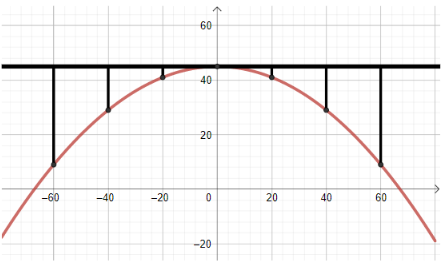
\includegraphics[scale=0.5]{parabelbrücke.png}
\end{minipage}

%---------------------------------------------------------
\question[6] % Barth Band 1 Kap 6.5 A18b
Für welchen Wert des Parameters $p$ berührt die Gerade $g$ die Parabel $p$ genau in einem Punkt?
\[p:y=x^2 \quad\text{ und }\quad g:y=p\*x-9\]


%---------------------------------------------------------
\question[2]
Bestimme die $x-$Koordinaten der Schnittpunkte der Parabel $p:y=4x+x^2$ mit der
Geraden $g:y=3x+\frac{3}{4}$.

%---------------------------------------------------------
\noaddpoints
\question[\totalpoints] %GZP23 A14
\addpoints
Gegeben sind die beiden Funktionen $f:y=3\*(x+4)^2-2$ und $g:y=-2.5x+2$.
\begin{parts}
	\part[2] Berechne die $x-$Koordinaten der Schnittpunkte der Graphen von $f$ und $g$.
	\part[2] Die Graphen von $f$ und $g$ werden an der $x-$Achse gespiegelt. Bestimme die Funktionsgleichungen der gespiegelten Graphen $f'$ und $g'$.
\end{parts}

%---------------------------------------------------------
\noaddpoints
\question[\totalpoints] %GZP24 A8
\addpoints
Gegeben sind die Parabel $p(x)=\frac{1}{2}x^2-2x+1$  und die Gerade $g(x)=-\frac{3}{4}x+4$
\begin{parts}
	\part[2] Berechne die $x-$Koordinaten der Schnittpunkte der Gerade mit der Parabel.
	\part[2] Gib die Gleichung einer zu $g$ parallelen Gerade an, welche die Parabel nur in einem Punkt
	berührt.
\end{parts}

%---------------------------------------------------------
\question[6] %Algebra 9/10 S112 A65b
\begin{minipage}{0.55\linewidth}
    Von einem $20$cm langen und $8$cm breiten Kartonstreifen werden die beiden schraffierten Flächen weg geschnitten und die vier Seitenflächen nach oben gefaltet. Nun entsteht eine oben offene Schachtel mit rechteckiger Grundfläche. Diese soll $15$ cm lang sein.
\end{minipage}
\hfill
\begin{minipage}{0.4\linewidth}
    \centering
    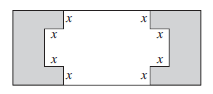
\includegraphics[scale=1]{extremalwert-schachtel.png}
\end{minipage}
\vspace{5pt}\\
Berechne die Höhe der Schachtel mit dem maximalen Volumen.

%---------------------------------------------------------
\question[6] %Barth Band 1 Kap 6.5 A16
\begin{minipage}{0.55\linewidth}
    Sie möchten an einer Ecke Ihres Hauses ein L-förmiges Blumenbeet anlegen, welches mit einem Gartenzaun  umrandet werden soll. Sie besitzen einen Gartenzaun der Gesamtlänge $50$ Metern. Wie müssen Sie $x$ und $y$ wählen, damit der Flächeninhalt des Blumenbeetes maximal wird? (Beachten Sie die in der Abbildung dargestellten speziellen Abmessungen des Beetes.)
\end{minipage}
\hfill
\begin{minipage}{0.4\linewidth}
    \centering
    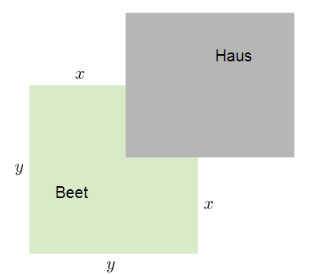
\includegraphics[scale=0.5]{extremalwert-blumenbeet.png}
\end{minipage}



\end{questions}
\end{document}